\chapter{Sparse Transformations}\label{chap:SparseRAJA}
\chapterabstract{
Performance portability libraries like RAJA and Kokkos are a growing approach to the maintainability problems of large applications. 
While these libraries can productively represent and efficiently execute many computations, they lack robust support for an important type: sparse computations. 
Sparse computations are widespread, present in the solvers of large simulation codes, economic optimization problems, search engines, and recommendation systems. 
While it is technically possible to implement some sparse computations in RAJA, users cannot write sparse codes in a way that respects the abstractions provided by RAJA to think about and program the problem, most importantly the abstractions of multi-dimensional data and loops.
Furthermore, changing the format of the sparse data becomes a porting task that touches every part of the code. 
Rather than relying on existing approaches to sparse computations, which use domain-specific languages and compilers to generate efficient implementations, my approach incorporates the abstractions into the RAJA library itself. 
RAJA already contains a strong separation of the components of a computation: the operation, data, iteration space, and schedule. 
The key idea of my approach is to treat the sparsity as its own component in the RAJA program. 

The challenges of this approach lie in achieving good performance without losing portability. 
Two emerge specifically: constructing / traversing a sparse iteration space and accessing data without using searches. 
For the problem of the iteration space and schedule, I use leader and follower iterators to represent and traverse sparse iteration spaces, built on the symbolic iteration space capabilities I developed to support dense triangular iteration spaces. 
This approach supports coordinate storage, and I show how it can be extended to support compressed row and column storage formats. 
To efficiently traversal of the sparse structures, I incorporate an expected next access cache, inspired by prefetching systems.

}

Sparse computations are important.

We need to be able to change sparse data formats, and changing sparse formats in handwritten code is more difficult than with dense.

There isn't a performance portable way in RAJA to change sparse formats.

Ideally, performance portable format changes would enable computations to access data using the same interface regardless of data format.

RAJA's existing multidimensional data interface is a convenient and intuitive target.

Conforming to this interface presents two challenges: traversing the iteration space and traversing the data.

Iteration space traversal is enabled by introducing new \verb.SparseSegment. abstractions.
Data traversal is enabled by incorporating incremental updates into the View's access function.

Algorithmic complexity suggests that this approach could compete with existing support.
Prototype performance evaluation suggests that the increased constant factor incurred by runtime overhead is too expensive, causing a $2-3\times$ slowdown.

The two largest sources of runtime overhead are extracting the iterator values from the segments (18\% of kernel execution) and the conditionals used in the incremental updates (8\% of kernel execution).

The key to reducing the runtime overhead is template specialization, but more specialization comes at the cost of the expressiveness and portability of the interface.

Extracting the iterator values could be specialized using RAJA's existing \verb.IndexSet. abstraction.
However, this sacrifices multi-dimensional loop abstractions and cannot support imperfectly nested loops.

Removing the conditionals in the incremental updates is possible using special iterator types.
This is only possible when the data is certain to be traversed in a specified order.

\todo{unclear if i've implemented the possible improvements}
\todo{paragraph that indicates what will be in each section}

\section{Sparse Computations And Data}


%Sparse computations are important.
Sparse computations --- those that operate on data where ``there is advantage to be taken of the percentage or distribution of zero elements''~\cite{duff1977survey} --- have long been a bottleneck for high performance computing applications. 
Even as early as 1971, scientists lamented the difficulty of computing with sparse data~\cite{willoughby1971sparse}.
More than fifty years later, while new application domains have garnered attention~\cite{he2016fusing,zhao2018bridging,zhu2019sparse}, programming sparse applications is still a challenge.
Many of these difficulties emerge from the variety of compression strategies used to avoid storing and computing on zero elements.


\begin{figure*}
  \centering
  \begin{subfigure}{0.45\textwidth}
    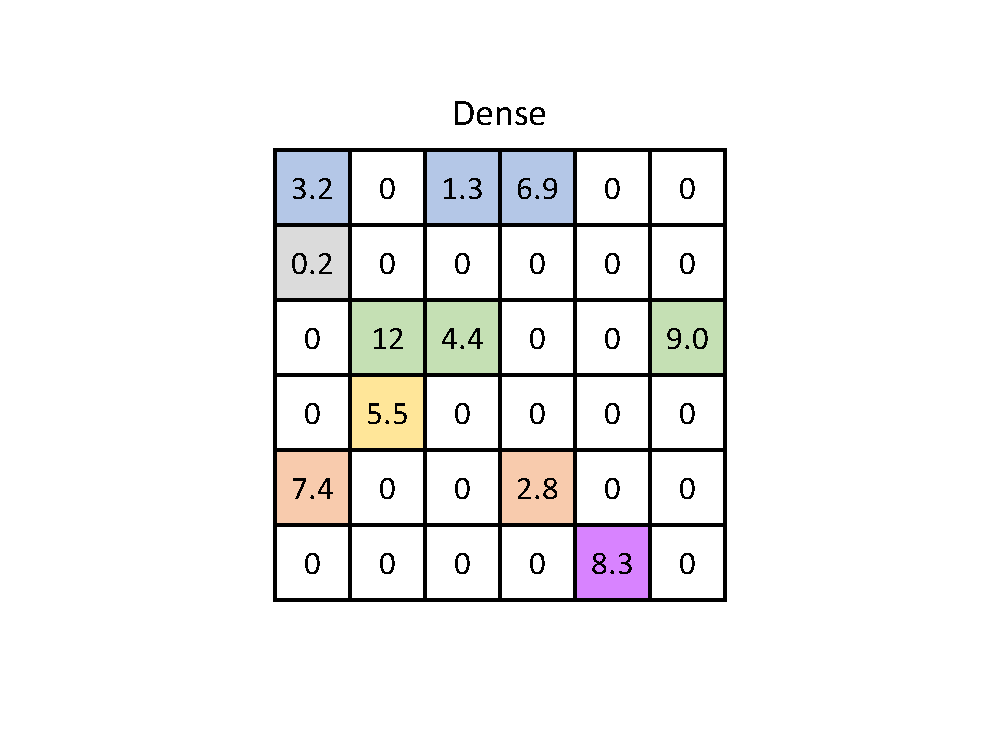
\includegraphics[page=1,width=\textwidth]{FormatDiagram.pdf}
    \caption{Dense representation of data. All entries are stored, including zeros.}\label{FormatDiagram:Dense}
  \end{subfigure}
  \begin{subfigure}{0.45\textwidth}
    \includegraphics[page=2,width=0.95\textwidth]{FormatDiagram.pdf}
    \caption{Coordinate storage (COO) representation of data. The nonzero entries and their corresponding index values are stored. Here, the entries are sorted by row index then by column index.}\label{FormatDiagram:COO}
  \end{subfigure}

  \begin{subfigure}[c]{0.45\textwidth}
    \includegraphics[page=3,width=0.95\textwidth]{FormatDiagram.pdf}
    \caption{Compressed sparse row (CSR) representation of data. Instead of storing duplicate row values, the row array is compressed to the offsets in the column and value arrays where each row starts.}\label{FormatDiagram:CSR}
  \end{subfigure}
\caption{Dense, COO, and CSR storage representations of the same data.  Nonzero entries are colored by their row value.}\label{FormatDiagram}
\end{figure*}

%We need to be able to change sparse data formats,
Like with dense codes, it is often desirable to change the sparse data format a computation uses.
Because of their compression strategies, sparse data structures usually do not support constant-time random access.
Instead, format and schedule are coordinated so that the sparse data is traversed in order, replacing random access with incremental updates.
This means that in addition to improving memory performance, a good choice of format can improve the algorithmic complexity of a program.
Changes in algorithm, schedule, machine, and input data all influence which format is best (see Section~\ref{sec:SparseFormats}).


%and changing sparse formats in handwritten code is more difficult than with dense.
However, more significant performance improvement comes at the cost of more significant refactoring.
With handwritten codes, changing the sparse format used in a loop nest can involve changes to every single line of code for the loop nest.
An example of this phenomenon is shown in Listing~\ref{DenseAndSparseMV}, which contains implementations of sparse matrix vector multiplication (SpMV) for three different formats.
This effect, already present with a simple kernel and commonplace formats, is amplified as the complexity of the loop nest and format increase.
Part of the problem here is that with dense data, no matter the layout, there is a closed form, $O(1)$ complexity function for calculating the location of any element.
With sparse formats, there is no constant-time random access.
Instead, the computation must be reorganized to stream through the sparse data, even if it means indirect accesses in dense data.
Because the computation is written around streaming through sparse data, most of the code ends up implementing the traversal of the nonzeros rather than the computation the programmer wants to express.

\begin{figure}
\begin{lstlisting}[caption={Matrix vector multiply routines for matrices in different formats.},label=DenseAndSparseMV]  
//Dense
void dense_matrix_vector_multiply(View2D A, View1D x, View1D y) {
  int Ni = A.num_rows();
  int Nj = A.num_cols();
  for(int i = 0; i < Ni; i++) {
    for (int j = 0; j < Nj; j++) {
      y(i) += A(i,j) * x(j);
    }
  }
}

//Coordinate storage
void COO_matrix_vector_multiply(COOView2D A, View1D x, View1D y) {
  int nnz = A.numNonZeros();
  for(int idx = 0; idx < nnz; idx++) {
    int i = A.rows(idx);
    int j = A.cols(idx);
    y(i) += A.vals(idx) * x(j);
  }
}

//Compressed Sparse Row
void CSR_matrix_vector_multiply(CSRView2D A, View1D x, View1D y) {
  int Ni = A.numRows();
  for(int i = 0; i < Ni; i++) {
    startIndex = A.rowptr(i);
    endIndex = A.rowptr(i+1);
    for(int j = startIndex; j < endIndex; j++) {
      y(i) += A.vals(j) * x(A.col(j));
    }
  }
}
\end{lstlisting}
\end{figure}

  
%There isn't a performance portable way in RAJA to change sparse formats.
In RAJA, while there is some support for representing sparse computations, there is not a performance portable way to change sparse formats.
The \verb.IndexSet. abstraction can be used to iterate over the coordinates of a sparse structures nonzero entries, but requires the loop nest to be flattened to a one-dimensional traversal.
For a perfectly nested, reorderable computation like SpMV, this is a manageable requirement.
For a computation with dependences and imperfect nesting, like Gauss-Seidel iterative solve, this requirement becomes much more troublesome.
Even after wrangling a computation into this representation, changing the format of the sparse data can mean modifying large swaths of code, both within the computation itself and in constructing its iteration space.

%Ideally, performance portable sparse format changes would enable computations to access data using the same interface regardless of data format.
%RAJA's existing multidimensional data interface is a convenient and intuitive target.
Ideally, performance portable sparse format changes would enable computations to access data using the same interface regardless of data format.
RAJA's existing multidimensional data interface is a convenient and intuitive target.
With this approach, the description of a sparse computation would look quite similar to a dense version.
In a similar vein, RAJA already contains an interface for representing a computation's schedule.
If support for sparse computations could be built using these existing abstractions, it would create significant programmability benefits.
The computation would be sparse, but it would look as if it were dense.
 
%Conforming to this interface presents two challenges: traversing the iteration space and traversing the data.
This chapter details the design decisions and lessons learned while developing a prototype of this approach.
Conforming to the existing interface of RAJA computations presents two challenges: constructing the iteration space and traversing the sparse data.
Iteration space construction is enabled by introducing new \verb.SparseSegment. abstractions.
Data traversal is enabled by incorporating incremental updates into the sparse View's access function.
These solutions were developed based on the need for flexible but performant interfaces.

Algorithmic complexity suggests that implementations using this approach could compete with implementations specialized for specific formats.
However, evaluation disproves this hypothesis, showing the increased constant factor incurred by runtime overhead is too expensive, causing a $1.5-2\times$ slowdown.
More aggressive optimization of the approach would come at the cost of restricting the class of sparse computations the approach could represent.
I conclude that RAJA's approach to decoupling data, iteration space, and schedule is sufficient for dense codes, but it cannot represent the more significant coupling of these elements present in sparse codes.

The rest of this chapter proceeds as follows.
Section~\ref{sec:SparseFormats} reviews the wide variety of sparse formats that have been developed and motivates the need to have the one codebase support multiple sparse formats.
Section~\ref{sec:IndexSets} reviews RAJA's existing capabilities for representing sparse computations and their limitations.
Section~\ref{sec:SparseRAJA} describes the design and implementation of a prototype extension to support format-independent computation descriptions in RAJA.
Section~\ref{sec:SparseEval} evaluates the prototype, and Section~\ref{sec:SparseDiscussion} discusses lessons learned and concludes.



\section{A Preponderance of Sparse Data Formats}\label{sec:SparseFormats}

\section{Writing Sparse Codes in RAJA}\label{sec:IndexSets}

\section{Prototype Design and Implementation}\label{sec:SparseRAJA}

\section{Evaluation}\label{sec:SparseEval}

\section{Discussion and Conclusion}\label{sec:SparseDiscussion}


\section{Sparse Computations and Data}

\subsection{What is a Sparse Computation? 2 Examples.}

``Sparse'' describes data, and through it, everything else.
A simple definition for sparse data is data where the nonzero density is less than 0.1 or conversely, where more than 90\% of the entries are zero.
Other definitions are slightly less clear cut but more useful, defining a sparse matrix as one where there is advantage to be taken of the percentage or distribution of zero elements~\cite{duff1977survey}.
In computations using this type of data, it is often meaningless to operate on the zero entries (e.g.\ summing).
Further, storing all the zeros is not usually feasible, or even possible.
Thus, methods of storing only the nonzero entries have been developed, two of which are shown in Figure~\ref{FormatDiagram}.

1.
Problems involving directed graphs, like those encountered in social networks or web page ranking, are often formulated as sparse computations. 
This is because they often use an adjacency matrix to represent the graph itself.
An adjacency matrix encodes in its entries the connections between nodes in the graph. 
For example, in a social network, if Alice follows Bob, information about this relationship would be stored in the matrix position indexed by $(Alice,Bob)$. 
Because most people in a social network are not connected to one another, most of the graph's adjacency matrix will be empty.
When seeking to analyze such a network, it would not make sense to store all the empty entries; storage is expensive.
Instead, the adjacency matrix can be stored using a sparse data format, which trades some flexibility in random access for storage savings.

2. 
In the realm of high performance computing, solving systems of linear equations is ubiquitous.
The systems of linear equations are often enormous, with a variable in the system for each point in the simulation's decomposition.
Importantly, each point in the simulation is connected to a limited number of other points, usually only the points directly around it.
This means that in the system's coefficient matrix, most entries will be zero, as the nonzero entries represent connections and relationships between different points.
Because of the compression strategies used to only store the nonzero values, more cycles are spent getting the necessary data into the CPU than in a dense computation.
To improve this situation, researchers have developed countless different storage formats, each geared towards different processor types, algorithms, and data characteristics.
A sparse format that is specialized for the characteristics of a social network may not be ideal for storing the data of a sparse system of equations.

\subsection{Challenges Writing Sparse Computations}

The list of sparse formats is seemingly endless, and a computation written for a particular format needs to be rewritten to use a different one.
There are general purpose formats like coordinate storage (COO) and compressed hyperplane storage (CHS)~\cite{ahmed2000compiling}, of which compressed sparse row (CSR)~\cite{gustavson1972some} and compressed sparse column (CSC) are instances.
There are banded formats, best for data with most entries clustered along the diagonal~\cite{jennings1966compact}, and jagged formats best for parallelized iterative algorithms~\cite{saad1989krylov,montagne2004optimal}.
There are formats specialized for GPUs~\cite{fan2004gpu,bell2009implementing,bell2008efficient,monakov2010automatically} and formats for FPGAs~\cite{sun2007sparse,kestur2012towards,fowers2014high}.
Then of course there are specializations to the general purpose formats, like doubly~\cite{buluc2008representation} --- or even triply~\cite{mofrad2019efficient} --- compressed sparse formats for data with many completely empty rows and blocked compressed sparse row~\cite{vuduc2005fast} for avoiding communication in distributed settings.

There have been many approaches to reduce the impact of this variety, generally falling into one of three categories: general sparse formats, standardized libraries, and sparse compilation.
General sparse formats allow for a uniform interface for sparse data, but fail to leverage valuable data characteristics to improve memory usage and arithmetic intensity.
Standardized solver libraries~\cite{eisenstat1977yale,eisenstat1977yale2,eisenstat1984new,kincaid1982algorithm,chu1980user,george1984new,marsten1981design,saad1990sparskit,falgout2006design} abstract away data traversal entirely, improving maintainability at the cost of requiring an application use its formats and functions.
Compilation approaches~\cite{ahmed2000compiling,ahmed2000framework,bik1993automatic,bik1996automatic,bik2022compiler} make writing code easy, and offer good performance, but support a limited range of computations and introduce build system complexities and fragilities.
Also, there is the cost of switching code to use that compiler's language instead of the one its already written in.

Each of these options suffers in either performance, productivity, or portability.
Performance portability libraries like RAJA~\cite{hornung2014RAJA}, Kokkos~\cite{edwards2014kokkos}, and YAKL~\cite{norman2022portable} strike a great balance here, but offer little support for sparse computations.
Most of the code ends up implementing the traversal of the data structures rather than the computation the programmer wants to express.
For example, many of the abstractions that a programmer would use to think about a computation, like multi-dimensional data and nested loops, do not transfer to the domain of sparse computation.
This is because they must program to the specific data format in use instead of their conceptual model of the computation.


\subsection{Contributions}

My approach explores the possibilities of incorporating some of the advances in sparse computations developed in previous approaches into a performance portability library, specifically those that generate efficient implementations from dense-looking specifications.
The approach builds on the strong separation of concerns present in the RAJA library, taking it a step further by treating the sparsity of the data as its own component.
By isolating the sparsity as its own concern, it becomes more straightforward to specify its structure, as well as how it interacts with the other components of a RAJA computation.
This technique ensures an extension to the library that is comprehensible, flexible, and aligned to the existing features and feel of RAJA\@.

One of the central challenges to this approach is that it lacks the code generation capabilities present in compiler approaches.
For example, a code generating approach can translate a format-agnostic description of a computation into an optimized implementation for a specific format.
The approach I develop here is limited to standard C++ features, meaning template instantiation is the only code generation feature available.
This poses a challenge.
Because loop bodies in RAJA are given as callable lambda functions, my approach cannot rewrite (or even directly inspect) the operations they perform.
This is in contrast with approaches that generate data accesses from the dense-looking specification and combine C++ metaprogramming with a restructuring compiler~\cite{ahmed2000compiling,ahmed2000framework}.
Instead, I use symbolic evaluation to perform analysis at runtime, then construct a sparse iteration space and incorporate a technique for efficient access directly into the call operator of the sparse data structure.

This chapter contains the following contributions:
\begin{itemize}
\item An interface for format-agnostic representation of sparse computations in the RAJA performance portability library.
\item An approach for the partial automation of the construction of a sparse iteration space.
\item An approach for efficient access of sparse data without requiring the code generation capabilities of compiler-based approaches
\item A prototype implementation of these components for two classes of sparse formats
\item An evaluation comparing the approach with hand-implemented variants specialized for coordinate storage formats.
\end{itemize}


\section{Design Considerations}

Unlike approaches that develop a entirely new system for supporting sparse computations, this approach is developed as part of an existing performance portability library.
This imposes novel constraints, namely that the extensions presented herein must \textit{build} on the existing abstractions, rather than replace or reformulate them.
Conveniently, RAJA already provides a strong separation of the components of a computation and an approachable interface for recomposing them.
This section presents versions of matrix vector multiplication to illustrate these features of RAJA and their limitations in expressing sparse computations.
Then, it argues from a computational complexity standpoint that with sufficient optimization, this approach can provide comparable performance to a hand-implemented version of the code.

\subsection{Matrix Vector Multiply, Dense and Sparse}

Listing~\ref{DenseAndSparseMV} shows C-like implementations of the SpMV kernel using dense and sparse data formats.
The first implementation shows the computation written for a dense matrix.
The second implementation shows the computation written for coordinate storage (COO). 
In this format, the View contains three vectors: one for the row indices, one for the column indices, and one for the nonzero values.
These vectors contain as many elements as there are nonzero values.
The third implementation shows the computation written for a View in compressed sparse row storage (CSR).
This storage format is based on COO, but rather than storing every element of the row vector, it is compressed to a vector of offsets that indicate the start of each row within the column and value vectors.
Figure~\ref{FormatDiagram} shows a graphical representation of the three formats.



Consider the extent to which the representations of the computations depend on the selected data format.
In the sparse implementation, the data format of \verb.A. changes not only the access to \verb.A., but also the bounds of the inner loop --- now a function of the entries of \verb.rowptr.--- and even the access to the other data in the computation (\verb.x.).
All parts of the computation description have been tied up with the format of just one of the arrays.
This means that changes to the format of \verb.A. will require modifying nearly all parts of the computation, significantly reducing the flexibility of the code.


\subsection{RAJA's Flavor of Decomposition}
The previous subsection showed how different sparse formats need to be handled when changing sparse formats by hand.  
In this subsection, I discuss RAJA's approach to decomposition and the constraints it places on my approach of providing a way to specify the sparse computation without having to rewrite the loops.

As discussed in previous chapters, a RAJA computation is broken up into a description of the operation, the iteration space, the schedule, and the data format.
The main idea of my approach is to introduce an additional component for the sparsity of the data.
Then, the problem of extending RAJA to support sparse computations is reduced to identifying how this new sparsity should interact with each of the existing components.

The operation of the computation is provided by the user as lambdas that execute the iterations of a loop. 
Because the operation involves accessing sparse data, it presents strong constraints on the design of the sparse extension. 
Most importantly, the operation of the loop nest should be written the same regardless of the format. 
The natural candidate here is the existing interface for data access in dense RAJA codes: the call operator. 
While using the call operator to support accesses to sparse data produces an attractive interface for describing a computation, it surfaces the challenge of devising an access function that traverses the sparse data efficiently throughout a computation. This problem and my solution are discussed in Section~\ref{sec:SparseAccess}.

For the iteration space, we take a similar approach of format-agnostic specification.
The programmer describes the iteration space as if its a dense code then use the sparsity of the data to exclude iteration space points that do not access nonzero data.
This can be partially automated as part of the construction of the computation object, or done ahead of time by the programmer.
The automated process involves using the access information extracted from the operation to determine which iteration space points need to be retained.

The approach of augmenting a dense-like specification continues into the description of the schedule. 
The central challenge here is related to the construction of the sparse iteration space. 
As the sparse space is created out of the dense one, its representation needs to be compact and easily traversable by RAJA's kernel execution. 

Finally is the data format, where the sparsity plays a greater role.
While I restrict the prototype to COO and CHS formats, the dimensional ordering still plays an important role.
This is because the particulars of the data storage order influence the efficiency of constructing the sparse iteration space and traversing through the data.
Regardless of the underlying representation, the layout of the sparse view supports the standard multi-dimensional indexing functions that are used to access dense data.

\subsection{Computational Complexity}

Even for computations that only executes iterations that access a nonzero value, application performance depends on the speed the sparse data can be accessed.
Without any optimizations, each access to sparse data requires searching. 
Each dimension in the index hierarchy must be searched for the corresponding value, until either the entry is found or it can be determined that the entry is a zero.
In the worst case, for a View with $D$ dimensions and $NNZ$ nonzero entries, the complexity of a single access is $O(D * \log(NNZ))$. 
This is compared to $O(D)$ for a dense View.

Requiring a search on every access to a sparse structure is prohibitively expensive, but it is possible to reduce the complexity to constant time.
Specifically, if the computation uses a schedule and format that access and store the data in exactly the same order, then the search can be avoided entirely.
Instead, the index into the View's data is updated incrementally, processing the data in order.

In implementations written by hand or with code-generating approaches, incremental updates are hard-coded into the loop's implementation, either by the programmer or the compiler.
Each format requires a unique implementation that traverses its entries in the appropriate order, so code written for one format will not work for another.
My approach incorporates parts of this incremental update technique without requiring the code to be rewritten for each desired format. 
This involves maintaining a field in the SparseView that tracks its most recent access.
Then, when accessed, the view checks if the indices are for the entry stored next in the data. 
If so, the view can bypass the searching and immediately return the desired value. 
If not, the view performs the search as to return the correct value. 
This approach, a sort of software prefetching, does incur the overhead of a comparison between the current access and the expected access, but this $O(D)$ check is much faster than the $O(D*\log(NNZ))$ search.
The hypothesis is that, with sufficient optimization, this approach can provide comparable performance to a hand-implemented version of the code.

\section{Constructing a Sparse Iteration Space}\label{sec:sparseIterspace}
Omitting unnecessary iterations is key to the performance of a sparse computation. 


The first performance barrier for SparseRAJA is the representation and construction of the sparse iteration space.
While individual dimensions in a RAJA iteration space can be ranges (using \verb.RangeSegment.) or arbitrary lists (using \verb.ListSegment.), dimensions can only be combined using the cartesian product. 
This presents a problem, as scarcely any sparse iteration spaces can be represented as a cartesian product.
Another option is needed, and here, I explore two.
\todo{more here about the range segment and list piece, but not current priority.}

\subsection{Option 1: Specialized Iterators}
The leader/follower iterator approach requires no changes to the kernel policy, but is limited in the scheduling orders in can support. 
At a high level, the iterators for each loop dimension are synchronized, traversing a zipped list rather than a cartesian product. 
Because this method incorporates the synchronization through the segments themselves, it does introduce some runtime overhead.

When constructing the sparse iteration space, the outermost segment is created as a \verb.LeaderSegment. object and the inner segments are created as \verb.FollowerSegment. objects.
The inner \verb.FollowerSegment. objects store a reference to the lead segment with which they will synchronize.
Using this reference, the follower segments instantiate inner loops of length one, containing only the value in the synchronized position. 
This has the effect of compressing the multi-dimensional loop nest into a 1 dimensional loop nest traversing all the dimensions together.

Note that in this form, the approach can only support perfectly nesting schedules.
This becomes clear with an example.
Consider the following code, which accumulates the row sums of a sparse matrix into the dense vector \verb.y..:
\begin{figure}
\begin{lstlisting}
using POLICY=KernelPolicy<
  statement::For<0,
    statement::Lambda<0>,
    statement::For<1,loop_exec,
      statement::Lambda<1>
    >
  >
>;

auto init_lam = [=](auto i) {
  y(i) = 0.0;
}
auto accum_lam = [=](auto i, auto j) {
  y(i) += A(i,j);
}

auto i_dim = LeaderSegment(  {0,0,1,2,4,4,4,7});
auto j_dim = FollowerSegment({1,8,0,2,3,4,7,9});

kernel<POLICY>(make_tuple(i_dim,j_dim), init_lam, accum_lam);
\end{lstlisting}
\end{figure}
The correct behavior of this loop would be to zero out \verb.y(0)., then add to it \verb.A(0,1). and \verb.A(0,8)..
Next, it would zero out \verb.y(1). and add to it \verb.A(1,0)..
This process should continue, summing one value into \verb.y(2)., three values into \verb.y(4)., and finally one value into \verb.y(7)..

However, using this version of the leader/follower formulation, a different behavior emerges.
Because all iterator incrementing happens in the leader segment's loop level, the contents of \verb.y. are zeroed each time.
\verb.y(0). is zeroed, then \verb.A(0,1). is added.
Then \verb.y(0). is zeroed and \verb.A(0,8). is added.
This repeats with each point in the iteration space, constantly overwriting the output. 
This problem can be resolved, using a refinement discussed in the subsection after next.

\subsection{Option 2: Loop Flattening}

The second option, loop flattening, approaches the problem from the direction of the kernel policy rather than the iteration space objects themselves.
Here, a new policy statement type is introduced: \verb.FlatFor.. 
It functions similarly to the \verb.For. statement policy, but rather than iteration a single segment, it iterates multiple simultaneously. 

Because this approach changes the kernel policy, a template parameter, it is less amenable to runtime modifications. 
Furthermore, it more strictly encodes the data layout into the schedule, making it more costly to change the computation to use a different format.
However, it would incur less overhead during kernel execution than the Leader/Follower Iterators approach, as it avoids the code associated with traversing the length one inner loop nests.

An additional drawback of this approach is that it only supports perfect nesting for the dimensions that it flattens. 
This means that a loop nest that uses additional statements to initialize data or write temporaries back to memory either before or after the second nesting level cannot be represented using the \verb.FlatFor. approach.
Because of these drawbacks, I use a modified leader/follower iterator approach in the prototype, but an approach that combines the two may be the most effective.

\subsection{Compressed Leader/Follower Iterators}

The chosen approach refines the basic leader/follower iterator approach and lays the foundation for supporting compressed formats like CSR and CSC.

Rather than doing all incrementing within the leader iterator and having the follower iterators traverse a length one segment, the leader segment compresses its dimension in the style of the CSR row pointer, and the follower iterators traverse variable length segments based on the number of nonzeros that share the same leader iterator value.
This modified approach essentially constructs the CSR compressed dimension as part of the execution.
This approach is perfect for loops that have initialization and finalization statements, such as the summing loop nest discussed above. 


\section{Traversing Sparse Data Efficiently}\label{sec:SparseAccess}\label{sec:EfficientTraversal}

Even with the iteration space reduced to only the necessary points, acceptable performance depends on traversing the sparse data structures efficiently without requiring a search on each access.
Here, the tradeoff is between flexibility in supporting types of computations and the performance benefits of more aggressive specialization.

\subsection{Option 1: ``Expected Next Access'' Cache}

The most flexible approach is something akin to software prefetching, based on the assumption that data will be accessed in order. 
With this approach, before an access reverts to a search of the sparse data, it checks if the current access is for the next nonzero in the View.
If so, it skips the search and immediately returns the value.
If not, it searches the View for the desired value.

While this approach incurs the cost of checking the access against the expected, it avoids the much more expensive cost of searching the entire data structure each time the View is read or written.
Additionally, it only needs a single access function, avoiding the type manipulation of the other options, and supports correct execution for all kernels, regardless of data access patterns.
Listing~\ref{expectedAccessImpl} shows a possible implementation of such an access function.
\begin{figure}
\begin{lstlisting}[caption={Possible implementation fo the Expected Next Access approach to efficient data traversal.},label=expectedAccessImpl]
ElementType access(auto i0, auto i1) {
  static int expectedIdx = 0;
  if (i0 == dims[0][expectedIdx] && i1 == dims[1][expectedIdx]) {
    return values[expectedIdx++];
  }
  
  entryIndex = search(i0,i1);
  if (entryIndex == -1) {
    return 0;
  } else {
    expectedIdx = entryIndex+1;
    return values[entryIndex];
  }
}
\end{lstlisting}
\end{figure}

This approach can also be used to skip searching on accesses to coordinates with zero values.
For example, if the current access is lexicographically greater than the previous access and lexicographically less than the expected one, it can be inferred that the access should return zero. This is useful in computations that make stencil accesses.

\subsection{Option 2: Specialized Traversal Layouts}
For a certain class of kernels, where there is only one access to a sparse View, and the schedule traverses that data in order, a different approach could remove the check present in the first approach.

In this approach, each format has two implementations. 
One implementation performs a random access search, while the other traverse the data in order. 
If a programmer indicates the data will be traversed in order, or the runtime system can prove that it will, the View can be switched to the fast access format before kernel execution.

This approach has the benefit of faster access times at the cost of a smaller domain of possible kernels it could support. 
For example, it could not support a kernel that makes two accesses to the same View or one that makes multiple traversals of the data, such as a matrix multiplication.

Abbreviated implementations of the formats are shown in Listing~\ref{specializedLayoutsImpl}.
\begin{figure}
\begin{lstlisting}[caption={Abbreviated format implementation for the Specialized Traversal Layout approach.},label=specializedLayoutsImpl]
class FastCOO {
  int currIdx = 0;
  \dots
  void preKernelLaunch() {
    currIdx = 0;
  }
  ElementType access(Idxs...indices) {
    return values[currIdx++];
  }
}
\end{lstlisting}
\end{figure}

\subsection{Option 3: Specialized Index Types}
The third option, like the second, uses an approach of dispatching to different access functions based on access pattern information.
Here, rather than using the View's layout type to select the access function, I use the type of the loop index values passed to the lambdas.
For example, the COO format may have two access functions, specialized for different inputs.
Listing~\ref{specializedIndexImpl} shows possible access functions fro the COO format.

This approach has the benefit of maintaining a single View layout type, avoiding the virtualization necessary to support the second approach.
This removes yet another source of overhead in the sparse access functions.
However, because it changes the type of the indexing variables, it imposes some of the same limitations as the symbolic evaluation functionality. 
Critically, all the data structures used in a kernel would need to support the different index types. 
For codes that only used dense and sparse Views, this is less of a problem.
For codes that access vectors or traditional arrays, this presents more serious issues.
Additionally, if two sparse Views are used in the same kernel, they both need to traverse their data in the efficient order.
This is because the same index type has to be used for both sparse Views.


\begin{figure}
\begin{lstlisting}[caption={Reference implementation for the Specialized Index Types approach.}, label=specializedIndexImpl]

ElementType access(int i0, int i1) {
  return searchAccess(i0,i1);
}
int fastIdx = 0;
ElementType access(FastIdx i0, FastIdx i1) {
  return values[fastIdx++];
}
\end{lstlisting}
\end{figure}

\subsection{Striking a Balance}
While the latter two options offer the potential for better performance than the first, it comes at a steep price of applicability.
For this reason, I use the expected next access approach in the prototype.
Certain computations present a challenge for all three approaches, such as the multiplication of a sparse matrix with its transpose.
Support for efficient traversal in such a computation is a direction for future research, and likely relies on maintaining multiple copies of the data structure, stored in different orders.
Such an approach could also maintain multiple expected access checks, one for each of the two storage directions.

\section{Prototype Implementation}
I implemented the approaches discussed in the previous two sections into a prototype for sparse computation support within RAJA\@.
Here, I discuss the interface and algorithms for constructing sparse data structures, iteration spaces, and computations.
% Constraints
% \begin{itemize}
% 	\item Conditional statements within loop bodies must not contain View accesses in their conditional expression.
% 	\item View indexing expressions must be lone iterators rather than affine expressions of the iterators, as in previous chapters.
% 	\item All writes to sparse Views must be updates, not insertions of new nonzeros.
% \end{itemize}

\subsection{Sparse Data Containers}

With the prototype's limitation to coordinate storage, two functions support the creation of sparse views: \verb.make_sparse_view. and \verb.make_permuted_sparse_view..
The former is a wrapper of the latter, generating a SparseView with the identity permutation.
For an $N$ dimensional SparseView, there are $N+2$ parameters to \verb.make_permuted_sparse_view..
The first $N$ parameters are vectors containing the index values for each dimension. 
This means that for a 2 dimensional SparseView, the first two arguments are the row and column indices of the entries.
The $N+1th$ parameter is a vector containing the entries themselves. 
Finally, the last parameter is the permutation vector for the SparseView. 
The idea of the permutation vector is that it changes how the entries of the view are sorted, but not how they are referenced / indexed.

Consider a sparse view containing the following entries, presented here unordered:
\begin{lstlisting}
DIM0: 0 1 2 1 0 2
DIM1: 1 1 0 2 2 0
DIM2: 1 0 2 1 0 0
VAL : A B C D E F 
\end{lstlisting}
If these entries are used to construct the standard SparseView, they will be reordered and stored as follows:
\begin{lstlisting}
DIM0: 0 0 1 1 2 2
DIM1: 1 2 1 2 0 0
DIM2: 1 0 0 1 0 2
VAL : A E B D F C
\end{lstlisting}
If the SparseView is constructed with the permutation vector $(2,0,1)$, they will be stored as:
\begin{lstlisting}
DIM0: 0 1 2 0 1 2
DIM1: 2 1 0 1 2 0
DIM2: 0 0 0 1 1 2
VAL : E B F A D C
\end{lstlisting}
Note that the list of dimensions is not permuted, only the order the entries are sorted. 
What this scheme means is that no matter the permutation, the access \verb.view(0,1,1). will always return \verb.A., even if its location in the list of entries changes.

The nonzero pattern of the SparseView data type is a read-only feature in the prototype.
This is not an inherent limitation, but additional considerations must be taken into account when designing mutable sparse data structures.
For example, because the iteration space of a sparse computation is based on the nonzero structure of the SparseView used in it, inserting new nonzeros into a SparseView during a computation could change the computation's iteration space as it is executing.
Additionally, the cost of inserting elements one at a time can be quite high. 
Thus, it is usually preferable to create a buffer of elements to insert and update the data structure all at once.
This buffer can take the form of a hash table which is emptied into the SparseView periodically.
With this in mind, it is possible to update the values of existing nonzero values within SparseViews, as this does not require inserting new elements into the data structure.

The SparseView class is templated by three values: the element type, the number of dimensions, and the type of the Format.
\verb.make_sparse_format. has an optional template parameter for choosing different formats, defaulting to coordinate storage.
The SparseView class wraps the templated sparse format type and manages a symbolic evaluation itself.
Most of its methods directly forward to calls of the format implementation class.
A programmer can easily create a new sparse format by creating an implementation class that implements a small collection of functions.
Most important is the call operator, but also necessary are functions for accessing individual dimension index values, the number of nonzero entries, and diagnostic functions for examining the expected access cache hit rates.

\subsection{Sparse Iteration Spaces}

The implemented algorithm for automatically constructing the sparse iteration space from the dense iteration space and a sparse data access addresses the common case.
It assumes the iteration space dimensionality and the data space dimensionality are equal, and is based on an access to the sparse data that uses each loop iterator once.


The idea of the algorithm is to construct the sparse iteration space out of the dimensions of the SparseView. 
First, the dimensions of the iteration space are matched to the dimensions of the SparseView based on the access information gathered from the symbolic evaluation.
For example, the accesses \verb.A(i,j). and \verb.A(j,i). match the first dimension of the SparseView to the first and second dimensions of the iteration space, respectively.
Second, using this mapping, the sparse iteration space segments are constructed.
The type of segment each View dimension is used to create is based on the kernel schedule.
This ensures that the lead segment is traversed by the outermost loop nest.
Listing~\ref{sparsifyAlg} shows a pseudo-code implementation of the algorithm.


\begin{figure}
\begin{lstlisting}[caption={Abbreviated algorithm for sparsifying a dense iteration space.}, label=sparsifyAlg]
auto sparsify(std::array<idx_t, NumDims> argumentOrder, 
              SparseView accessedView, Tuple nestingOrder) {
  viewDimIdx_to_iterDimIdx = argumentOrder;
  iterDimIdx_to_viewDimIdx = invert(argumentOrder);

  leadIterDimIdx = camp::get<0>(nestingOrder);
  followIterDimIndices = slice<1,NumDims>(nestingOrder);

  leadViewDimIdx = iterDimIdx_to_viewDimIdx[leadIterDimIdx];
  followViewDimIndices = apply(iterDimIdx_to_viewDimIdx, followIterDimIndices);

  viewSortOrder = [leadViewDimIdx,followViewDimIndices...];
  accessedView.sort(viewSortOrder);

  sparseIterSpace = [];
  for iterDimIdx in 0..NumDims {
    viewDimIdx = iterDimIdx_to_viewDimIdx[iterDimIdx];
    if(viewDimIdx == leadViewDimIdx) {
      currDim = LeadSparseSegment(view.dims[viewDimIdx])
      sparseIterSpace.push_back(currDim);
    } else {
      currDim = FollowSparseSegment(view.dims[viewDimIdx]);
      sparseIterSpace.push_back(currDim);
    }
  }
  return sparseIterSpace;
}
\end{lstlisting}
\end{figure}

\subsection{Sparse Kernel Objects}

The automatic construction of a sparse iteration space is surfaced to the user through the \verb.make_sparse_kernel. function.
An extension of the existing \verb.make_kernel. function, the sparse variant includes two extra parameters (one optional, one required) used to construct the sparse iteration space.
First is the required runtime parameter for the sparse View that the iteration space should be constructed around.
This parameter comes after the dense iteration space and before the lambdas for the loop bodies.
Second is an optional template index parameter, specifying which of the lambdas should be evaluated symbolically to gather the access information necessary for creating the new iteration space.
An abbreviated implementation is shown in Listing~\ref{makeSparseKernelAlg}.

When called, \verb.make_sparse_kernel. starts by symbolically evaluating the specified lambda.
This collects all access information, for both sparse and dense Views.
The next step isolates the accesses to the sparse View guiding the construction by a standard search.
This access, the kernel policy, and the dense iteration space are then used to construct the sparse iteration space.
The final step is to return a KernelWrapper that will execute the computation over the newly constructed sparse iteration space.

\begin{figure}
\begin{lstlisting}[caption={Abbreviated implementation of the function for creating a computation that automatically constructs the sparse iteration space.}, label=makeSparseKernelAlg]
template <typename KernelPolicy, idx_t SymExecLamIdx=0>
auto make_sparse_kernel(auto denseSegs, auto sparseView, auto loopBodyTuple) {
  auto symExecLambda = get<SymExecLamIdx>(loopBodyTuple);
  auto allAccesses = symbolically_evaluate(symExecLambda);
  auto sparseAccess = findAccessTo(sparseView, allAccesses);

  auto sparseSegs = make_sparse_iteration_space<KernelPolicy>(denseSegs, 
  sparseAccess);

  return make_kernel<KernelPolicy>(sparseSegs, loopBodyTuple);
}
\end{lstlisting}
\end{figure}

Alternatively, the programmer can construct the sparse iteration space themselves, then use the standard \verb.make_kernel. to generate the computation over the sparse iteration space.

\section{Evaluation}\label{sec:sparseEval}
To evaluate the prototype, I compare the performance of different versions of two benchmarks: sparse matrix vector multiplication (SpMV) and Gauss-Seidel iteration (GauSei).
The first version, \dense, implements the computation on dense data. 
The second version, \specialized, is specialized for a particular sparse format by hand. 
The third version, \sparseraja, implements the computation using the prototype support described above.
In terms of representation, the expectation is that the \dense{} and \sparseraja{} versions of the code will look similar, both varying significantly from the format-specific implementation of the \specialized{} version.
In terms of performance, the \dense{} version is expected to be the outlier, as it executes many more iterations than the \sparseraja{} and \specialized{} versions.

The evaluation process here is iterative, progressing through a loop of running the evaluation, profiling using hpctoolkit~\cite{adhianto2010hpctoolkit}, identifying potential optimizations, and implementing them. 
This is in service of evaluating the overall question of the feasibility of achieving comparable performance to the hand-specialized variants.


\subsection{Benchmark 1: SpMV}
While a relatively simple computation on its own, sparse matrix vector multiplication (SpMV) is a foundational building block for sparse computations.
The computation has two pieces of input data: a sparse matrix \verb.A. and a dense vector \verb.x.. 
Each element of the single output vector \verb.y. is the dot product of the corresponding row of \verb.A. with the whole vector \verb.x..
Listings~\ref{DenseMV},~\ref{SpecializedMV}, and~\ref{SparseRAJAMV} show the reference implementations for the three versions of the computation.

\subsection{Benchmark 2: Gauss-Seidel Iteration}

The second kernel, Gauss-Seidel iterative solve, is a well-known kernel for approximating the solution to a linear system.
The problem of solving a linear system is thus: given a coefficient matrix $A$ and a right-hand side vector $b$, find a vector $x$ such that $Ax=b$.
The Gauss-Seidel method does this by starting with an initial guess and successively refining it to closer and closer approximations.
This process is repeated until a desired level of accuracy is reached.

While the kernel itself is applied iteratively to refine the approximation, we focus here on the operations of the iterations internal to the kernel.
An imperfectly nested, two-dimensional loop nest, GauSei updates each element of the solution vector $x$ in sequence.
First, the dot product of a row of $A$ and the current approximation is accumulated in a temporary variable.
Note that if the approximation is exactly correct, this value will be equal to the corresponding entry of $b$. 
The difference between the temporary and the right-hand side is then used to update the approximation, and the process repeats.

Gauss-Seidel is a tricky kernel because of its data dependences.
The results of earlier iterations change values used in subsequent ones, meaning that the order of the iterations cannot be changed arbitrarily. 
For this reason, GauSei cannot be represented as tensor algebraic expressions, placing it outside TACO's space of expressible computations~\cite{}.

Listings~\ref{DenseGauSei},~\ref{SpecializedGauSei}, and~\ref{SparseRAJAGauSei} show the three reference implementations of the GauSei kernel.
Because of the significant variations between the three implementations, I also show a C-like reference implementation in Listing~\ref{CppGauSei}.

One such variation appears in the \specialized{} version. 
Because specializing the implementation for the COO format flattens the iteration space from two dimensions to one, guard statements must be inserted to check for changes in rows. 
Furthermore, it also requires pulling part of the final iteration out of the loop.

\subsection{Performance Results}

\subsubsection{SpMV}
\begin{figure}
  \begin{subfigure}{0.49\columnwidth}
    \includegraphics[width=\columnwidth]{SpMV_lines_perf.pdf}
    \caption{Execution times for Specialized and SparseRAJA variants at different sparse matrix densities. Lower is better. Both axis are log scale.}\label{SpMVExecTime}
  \end{subfigure}
  \hspace{0.02\columnwidth}
  \begin{subfigure}{0.49\columnwidth}
    \includegraphics[width=\columnwidth]{SpMV_ratios_perf.pdf}
    \caption{Overhead ratio between SparseRAJA and Specialized variants. Lower values indicate lower relative overhead for the SparseRAJA variant.}\label{SpMVRatios}
  \end{subfigure}
  \caption{Performance results for \SpMV{} benchmark. For low densities, the constant overhead causes a large performance discrepancy that levels off to around 2 for higher densities.}\label{SpMVPerformance}
\end{figure}

With the first version, the \sparseraja{} variant showed a geometric mean speedup of 0.103, just under a $10\times$ slowdown compared to the \specialized{} variant.
Analysis with hpctoolkit uncovered two opportunities for optimization.
The first was an expensive vector allocation. 
Using a fixed size array instead of a vector, performance was more than doubled to a mean speedup of 0.282, just under a $4\times$ slowdown.
Using the compressed leader iterator instead of the standard one further improved performance to its current mean speedup of $0.404$, about a $2.5\times$ slowdown.




\subsubsection{GauSei}
\begin{figure}
  \begin{subfigure}{0.49\columnwidth}
    \includegraphics[width=\columnwidth]{GauSei_lines_perf_COO.pdf}
    \caption{Execution times for Specialized and SparseRAJA variant using COO format at different sparse matrix densities. Lower is better. Both axis are log scale.}\label{GauSeiExecTimeCOO}
  \end{subfigure}
  \hspace{0.02\columnwidth}
  \begin{subfigure}{0.49\columnwidth}
    \includegraphics[width=\columnwidth]{GauSei_ratios_perf_COO.pdf}
    \caption{Overhead ratio between SparseRAJA and Specialized variants using COO format. Lower values indicate lower relative overhead for the SparseRAJA variant.}\label{GauSeiRatioCOO}
  \end{subfigure}
  \caption{Performance results for the \GauSei{} benchmark using the COO storage format. }\label{GauSeiPerfCOO}
\end{figure}


Figure~\ref{GauSeiPerfCOO} shows the initial performance of the SparseRAJA implementation using the COO storage format.
Figure~\ref{GauSeiRatioCOO} shows the ratio of the SparseRAJA variant execution time to the specialized variant execution time.
The geometric mean speedup of the SparseRAJA version relative to the specialized version is $0.364$, just under a $3\times$ slowdown. 
From the early profiling rounds of the \GauSei{} kernel, nearly 90\% of the execution time is spent in the SparseView's search-based random access function.
This is caused by the comparatively low expected access cache hit rate, driven by the irregular access patterns in the kernel.
First, each of the diagonal entries is skipped during the execution of the inner loop nest.
After each diagonal iteration, where no access is made because the conditional is false, the expected access is still the diagonal entry. 
Thus, the following iteration will access the entry after the diagonal and have to search.
Second, each diagonal is accessed after the row is processed in the finalizing statement.
This causes two misses, one when the finalizing statement executes and the access to the diagonal entry is made, then another on the first inner iteration of the next row, attempting to access the first entry of the row.
Barring the occasional circumstance where the diagonal is the last or only value in the row, there are three misses for each row in the input matrix.

Here we encounter a situation where a different data format would be beneficial.
For example, a format that additionally stores a vector of the diagonal entries separately from the other entries.
On an access, if the access is for a diagonal, it indexes directly into the vector, otherwise following the usual pattern of prefetching and searching.
Figure~\ref{GauSeiPerfDIAG} shows the performance of a variant using this DIAG storage format instead of the general COO format compared to the specialized hand-implemented variant.
Here, the geometric mean speedup is $0.460$, about a $2.2\times$ slowdown compared to the hand-implemented version.
This reduction in the overhead is a result of an improved access cache hit rate with the DIAG format.

\begin{figure}
  \begin{subfigure}{0.49\columnwidth}
    \includegraphics[width=\columnwidth]{GauSei_lines_perf_DIAG.pdf}
    \caption{Execution times for Specialized and SparseRAJA variant using DIAG format at different sparse matrix densities. Lower is better. Both axis are log scale.}\label{GauSeiExecTimeDIAG}
  \end{subfigure}
  \hspace{0.02\columnwidth}
  \begin{subfigure}{0.49\columnwidth}
    \includegraphics[width=\columnwidth]{GauSei_ratios_perf_DIAG.pdf}
    \caption{Overhead ratio between SparseRAJA and Specialized variants. Lower values indicate lower relative overhead for the SparseRAJA variant.}\label{GauSeiRatioDIAG}
  \end{subfigure}
  \caption{Performance results for the \GauSei{} benchmark using the DIAG storage format. The larger relative overhead for lower densities is due to access cache misses when a row only contains a diagonal entry.}\label{GauSeiPerfDIAG}
\end{figure}


\subsection{Avenues for Further Optimization}

Overall, the approach shows some promise.
Future optimization must target the specialization of as much of the computation as possible, especially the SparseView access functions and the extraction of iterator values from SparseSegments.
RAJA, and performance portability libraries more generally, excel when the C++ compiler is able to do as much as possible ahead of time.
Specifically, template specialization and optimization of the resulting code are important.
This is why RAJA is able to support writing dense codes with such low overhead.
Kernel execution uses the kernel policy template argument to instantiate a loop nest implementing the policy.
Then, aggressive inline and other automatic loop optimizations can further improve performance.

With SparseRAJA, overhead emerges as a result of the parts of the code where this specialization and optimization cannot occur.
One example of this is the 18\% of \GauSei{} kernel execution time spent extracting the values to pass to the loop body lambdas.
Because the Segment and Iterator types are virtualized, their use incurs overhead due to dynamic dispatch.
These types could be devirtualized using the curiously recurring template pattern (CRTP).
Further optimizations to this part of the system could reduce the cost of each extraction by pre-computing and storing offsets within the FollowSegments.
This could avoid references to the LeadSegment on many iterations.

A second example is the time spent in the SparseView access methods.
Simple optimizations, like switching the order of the expected access and diagonal checks were alone able to reduce the time spent here from 19\% of kernel execution time to 8\%.
This remaining 8\% is spent comparing expected index values, which could be reduced using one of the other techniques discussed in Section~\ref{sec:EfficientTraversal} that use specialization to remove the checks entirely.  


\section{Conclusion}

This chapter explored incorporating support for sparse computations and data formats into the RAJA performance portability library.
By treating the sparsity of the data as an independent component of the computation's specification, the approach enables concise and format-independent programming. 
Additionally, new sparse formats can be prototyped and incorporated into computations while changing only the declaration of the data.
However, the overhead of maintaining and updating the necessary data structures for kernel execution, especially updating the sparse iterative values, caused performance to suffer.
While this approach may be feasible as a foundation for introducing schedule and data transformations for sparse computations, future work will have to bring the performance of the system within the range of hand-implemented versions.





\begin{figure}
  \begin{lstlisting}[caption={RAJA implementation of dense matrix vector multiplication.},label=DenseMV]
  DenseView<1> x(Nj);
  DenseView<1> y(Ni);
  DenseView<2> A(Ni,Nj);
  
  using POLICY = KernelPolicy<
    statement::For<0,loop_exec,
      statement::For<1,loop_exec,
        statement::Lambda<0>
      >
    >
  >;
  
  auto seg1 = RangeSegment(0,Ni);
  auto seg2 = RangeSegment(0,Nj);
  auto segs = make_tuple(seg1, seg2);
  
  auto lam = [&](auto i, auto j) {
    y(i) += A(i,j) * x(j);
  };
  
  auto knl = make_kernel<POLICY>(segs, lam);
  knl();
  \end{lstlisting}
  \end{figure}
  \begin{figure}
  \begin{lstlisting}[caption={RAJA implementation of sparse matrix vector multiplication, specialized for COO storage.},label=SpecializedMV]
  DenseView<1> x(Nj);
  DenseView<1> y(Ni);
  DenseView<1> A_cols(NumNonZeros);
  DenseView<1> A_rows(NumNonZeros);
  DenseView<1> A_vals(NumNonZeros);
  
  auto seg = RangeSegment(0,NumNonZeros);
  
  auto lam = [&](auto idx) {
    auto i = A_rows(idx);
    auto j = A_cols(idx);
    y(i) += A_vals(idx) * x(j);
  };
  
  auto knl = make_forall<loop_exec>(seg, lam);
  knl();
  \end{lstlisting}
  \end{figure}
  \begin{figure}
  \begin{lstlisting}[caption={Implementation of SpMV using the SparseRAJA prototype},label=SparseRAJAMV]
  DenseView<1> x(Nj);
  DenseView<1> y(Ni);
  SparseView<2> A(Ni,Nj);
  
  using POLICY = KernelPolicy<
    statement::For<0,loop_exec,
      statement::For<1,loop_exec,
        statement::Lambda<0>
      >
    >
  >;
  
  auto seg1 = RangeSegment(0,Ni);
  auto seg2 = RangeSegment(0,Nj);
  auto dense_segs = make_tuple(seg1, seg2);
  
  auto lam = [&](auto i, auto j) {
    y(i) += A(i,j) * x(j);
  }
  
  auto knl = make_sparse_kernel<POLICY>(dense_segs, A, lam);
    
  knl();
  \end{lstlisting}
  \end{figure}
  

  \begin{figure}
    \begin{lstlisting}[caption={C-like version of Gauss-Seidel iteration},label=CppGauSei]
    View<2> A(N,N);
    View<1> b(N);
    View<1> x(N) = initial_guess;
    double temp;
    
    while(!has_converged()) {
      for(int i = 0; i < N; i++) {
        temp = 0.0;
        for(int j = 0; j < N; j++) {
          if (j != i) {
            temp += A(i,j) * x(j);
          }
        }
        x(i) = (b(i) - temp) / A(i,i);
      }
    }
    \end{lstlisting}
    \end{figure}
    
    \begin{figure}
    \begin{lstlisting}[caption={\dense{} version of Gauss-Seidel iteration},label=DenseGauSei]
    View<2> A(N,N);
    View<1> b(N);
    View<1> x(N) = initial_guess;
    double temp;
    
    using POLICY = KernelPolicy<
      statement::For<0,loop_exec,
        statement::Lambda<0>,
        statement::For<1,loop_exec,
          statement::Lambda<1>,
        >,
        statement::Lambda<2>
      >
    >;
    
    auto lam1 = [&](auto i) {
      temp = 0.0;
    };
    auto lam2 = [&](auto i, auto j) {
      if (j != i) {
        temp += A(i,j) * x(j);
      }
    };
    auto lam3 = [&](auto i) {
      x(i) = (b(i) - temp) / A(i,i);
    }
    
    auto seg1 = RangeSegment(0,N);
    auto seg2 = RangeSegment(0,N);
    auto segs = make_tuple(seg1, seg2);
    
    auto knl = make_kernel<POLICY>(segs, lam1, lam2, lam3);
    
    while (!has_converged()) {
      knl();
    }
    \end{lstlisting}
    \end{figure}
    
    \begin{figure}
    \begin{lstlisting}[caption={\specialized{} version of Gauss-Seidel iteration},label=SpecializedGauSei]
    View<2> A_rows(NNZ);
    View<2> A_cols(NNZ);
    View<2> A_vals(NNZ);
    View<1> b(N);
    View<1> x(N) = initial_guess;
    
    while (!has_converged()) {
      int prev_i = 0;
      double temp = 0.0;
      for(int idx = 0; idx < NNZ; idx++) {
        int i = A_rows(idx);
        int j = A_cols(idx);
        double v = A_vals(idx);
    
        if (i != prev_i) {
          double prev_diagonal = find(prev_i, prev_i, A_rows, A_cols, A_vals);
          x(prev_i) = (b(prev_i) - temp) / prev_diagonal;
          temp = 0.0;
          prev_i = i;
        }
        if (j != i) {
          temp += v * x(j);
        } 
      }
      double prev_diagonal = find(prev_i, prev_i, A_rows, A_cols, A_vals);
      x(prev_i) = (b(prev_i) - temp) / prev_diagonal;
    }
    \end{lstlisting}
    \end{figure}
    
    
    \begin{figure}
    \begin{lstlisting}[caption={\sparseraja{} version of Gauss-Seidel iteration},label=SparseRAJAGauSei]
    SparseView<2> A(N,N);
    View<1> b(N);
    View<1> x(N) = initial_guess;
    double temp;
    
    using POLICY = KernelPolicy<
      statement::For<0,loop_exec,
        statement::Lambda<0>,
        statement::For<1,loop_exec,
          statement::Lambda<1>
        >,
        statement::Lambda<2>
      >
    >;
    
    auto lam1 = [&](auto i) {
      temp = 0.0;
    };
    auto lam2 = [&](auto i, auto j) {
      if (j != i) {
        temp += A(i,j) * x(j);
      }
    };
    auto lam3 = [&](auto i) {
      x(i) = (b(i) - temp) / A(i,i);
    };
    
    auto seg1 = RangeSegment(0,N);
    auto seg2 = RangeSegment(0,N);
    auto segs = make_tuple(seg1, seg2);
    
    auto knl = make_sparse_kernel<POLICY, 1>(segs, A, lam1, lam2, lam3);
    
    while (!has_converged()) {
      knl();
    }
    \end{lstlisting}
    \end{figure}

    \begin{figure}
      \begin{lstlisting}[caption={C++ reference implementation of incomplete Cholesky factorization.},label=CppInCholFact]
      
      View<2> A(N,N);   
      
      for(i0 = 0; i0 < N; i0++) {
        A(i0,i0) = sqrt(A(i0,i0));
        for(i1 = i0+1; i1 < N; i1++) {
          if (A(i1,i0) != 0) {
            A(i1,i0) /= A(i0,i0);
          }
        }
        for(i1 = i0+1, i1 < N; i1++) {
          for(i2 = i1; i2 < N; i2++) {
            if (A(i2,i1) != 0) {
              A(i2,i1) -= A(i2,i0) * A(i1,i0);
            }
          }
        }
      }
      
      for(i0 = 0; i0 < N; i0++) {
        for(i1 = i0+1; i1 < N; i1++) {
          A(i0,i1) = 0;
        }
      }
      \end{lstlisting}
      \end{figure}